\chapter{結論}
\section{AIによる楽曲制作の結果}
\subsection{モデルによる生成結果の違い}
学習モデルごとの生成結果は単音の単純な羅列が続くbasic\_rnnに比べlookback\_rnnやattention\_rnnの方がリズム的な繰り返しが多いという特徴が見られた.
また,lookback\_rnnに比べattention\_rnnの方がの方が単純な繰り返しではなく,展開的な繰り返しをした.図\ref{fig:学習モデルごとの生成結果}はその生成結果である.(GarageBand上のスクリーンショット)
\begin{figure}[h]
    \begin{screen}
    \begin{center}
        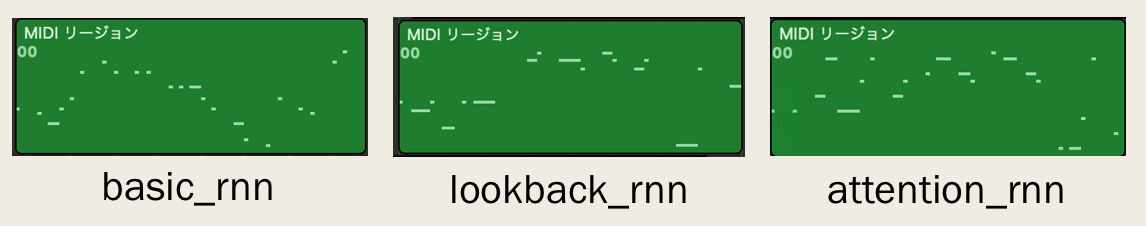
\includegraphics[scale=0.68, clip]{./img/model.png}
        \caption{学習モデルごとの生成結果}
        \label{fig:学習モデルごとの生成結果}
    \end{center}
    \end{screen}
\end{figure}
\newpage
\subsection{学習回数による生成結果の違い}
学習回数ごとの生成結果では,学習回数が増えるごとに学習させた楽曲に近づいた.また学習回数が少ないとコードのスケール外の音も入ってしまっていたが,学習回数を上げるとその現象の発生があまり起きなかった.図\ref{fig:basic_rnnによる学習回数ごとの生成結果},図\ref{fig:lookback_rnnによる学習回数ごとの生成結果},図\ref{fig:attention_rnnによる学習回数ごとの生成結果}はその生成結果である.(GarageBand上のスクリーンショット)
\begin{figure}[h]
    \begin{screen}
    \begin{center}
        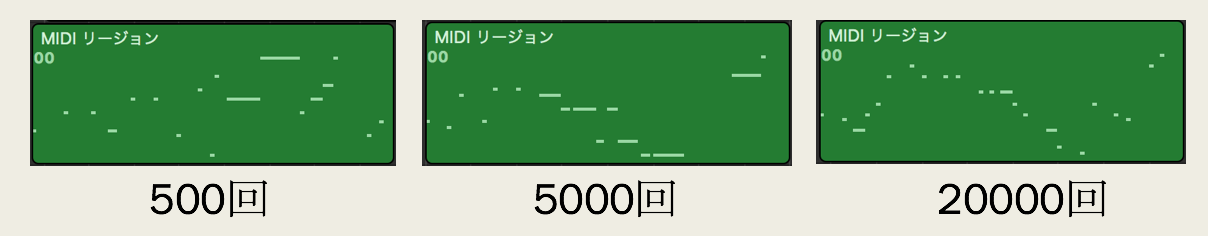
\includegraphics[scale=0.68, clip]{./img/basicMIDI.png}
        \caption{basic\_rnnによる学習回数ごとの生成結果}
        \label{fig:basic_rnnによる学習回数ごとの生成結果}
    \end{center}
    \end{screen}
\end{figure}
\begin{figure}[h]
    \begin{screen}
    \begin{center}
        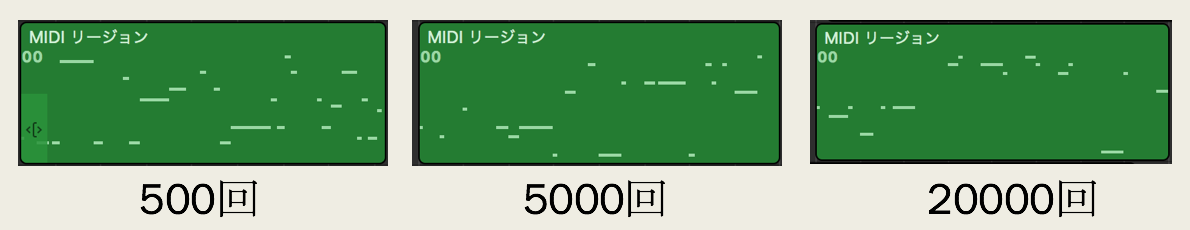
\includegraphics[scale=0.68, clip]{./img/lookbackMIDI.png}
        \caption{lookback\_rnnによる学習回数ごとの生成結果}
        \label{fig:lookback_rnnによる学習回数ごとの生成結果}
    \end{center}
    \end{screen}
\end{figure}
\begin{figure}[h]
    \begin{screen}
    \begin{center}
        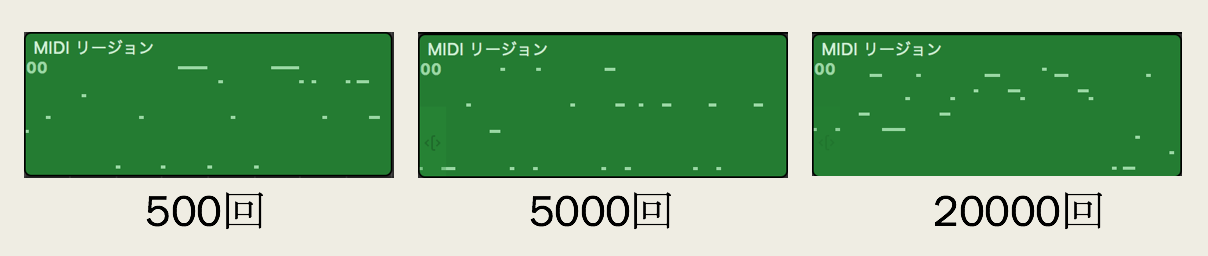
\includegraphics[scale=0.68, clip]{./img/attentionMIDI.png}
        \caption{attention\_rnnによる学習回数ごとの生成結果}
        \label{fig:attention_rnnによる学習回数ごとの生成結果}
    \end{center}
    \end{screen}
\end{figure}
\newpage
\subsection{ノード数による生成結果の違い}
ノード数による生成結果ではノード数32と64に比べ128の方が長い音が増えた.また音階にまとまりが出てあまり高音や低音に移動せず一定の音域の楽曲になった.図\ref{fig:ノード数ごとの生成結果}はその生成結果である.(GarageBand上のスクリーンショット)
\begin{figure}[h]
    \begin{screen}
    \begin{center}
        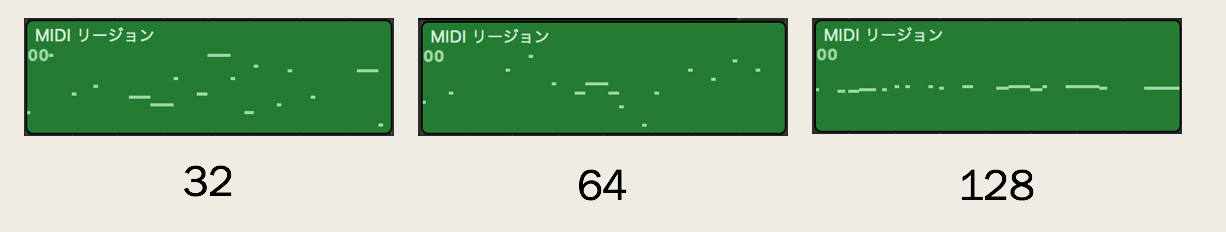
\includegraphics[scale=0.68, clip]{./img/nodo.png}
        \caption{ノード数ごとの生成結果}
        \label{fig:ノード数ごとの生成結果}
    \end{center}
    \end{screen}
\end{figure}
\newpage
\section{調査結果}
楽曲制作に関して有用な条件をアンケート形式で調査した.調査方法は学習回数が500回,5000回,20000回のそれぞれで生成したbasic\_rnn,lookback\_rnn,attention\_rnnの生成結果,basic\_rnn,lookback\_rnn,attention\_rnnそれぞれで生成したの学習回数500回,5000回,20000回での生成結果,basic\_rnnで生成したノード数32,64,128での生成結果
をそれぞれ視聴してもらい,それぞれの項目から一番良いと思うものを選択してもらう形式をとった.\\
 調査の様子を図\ref{fig:調査の様子}に示す.
\begin{figure}[h]
    \begin{screen}
    \begin{center}
        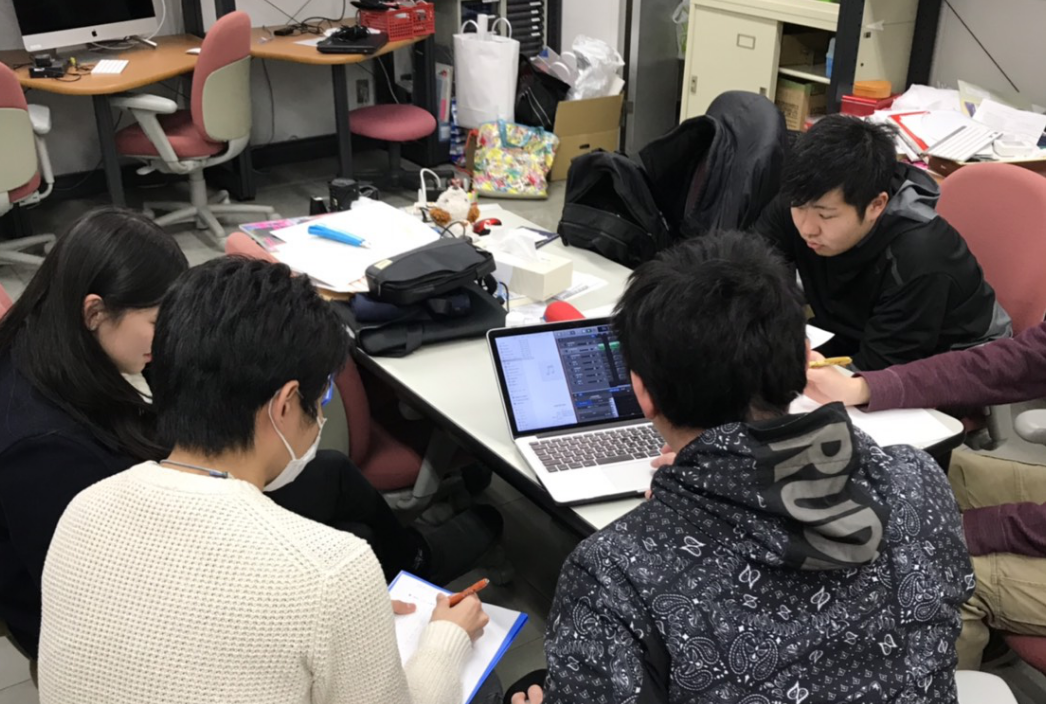
\includegraphics[scale=0.7, clip]{./img/tyousa1.png}
        \caption{調査の様子}
        \label{fig:調査の様子}
    \end{center}
    \end{screen}
\end{figure}
\newpage
\subsection{学習回数ごとの各モデルの調査結果}
学習回数ごとの各モデルの調査では学習回数が500回,5000回でlookbacl\_rnnが一番良いと答えた人の割合が半数を超えた.これはlookback\_rnnのモデルが繰り返しに対応していることで人間が聴きやすい楽曲になったことが考えられる.一方で学習回数20000回では全てのモデルの良いと答えた人の割合が同数だった.
これは学習回数を多くすることでスケール外の音が入るなどの現象がなくなり,生成される楽曲が似てくるためであると考えられる.\\
 以下の図\ref{fig:学習回数ごと各モデルの調査結果}に学習回数ごと各モデルの調査結果を示す.
\begin{figure}[h]
    \begin{screen}
    \begin{center}
        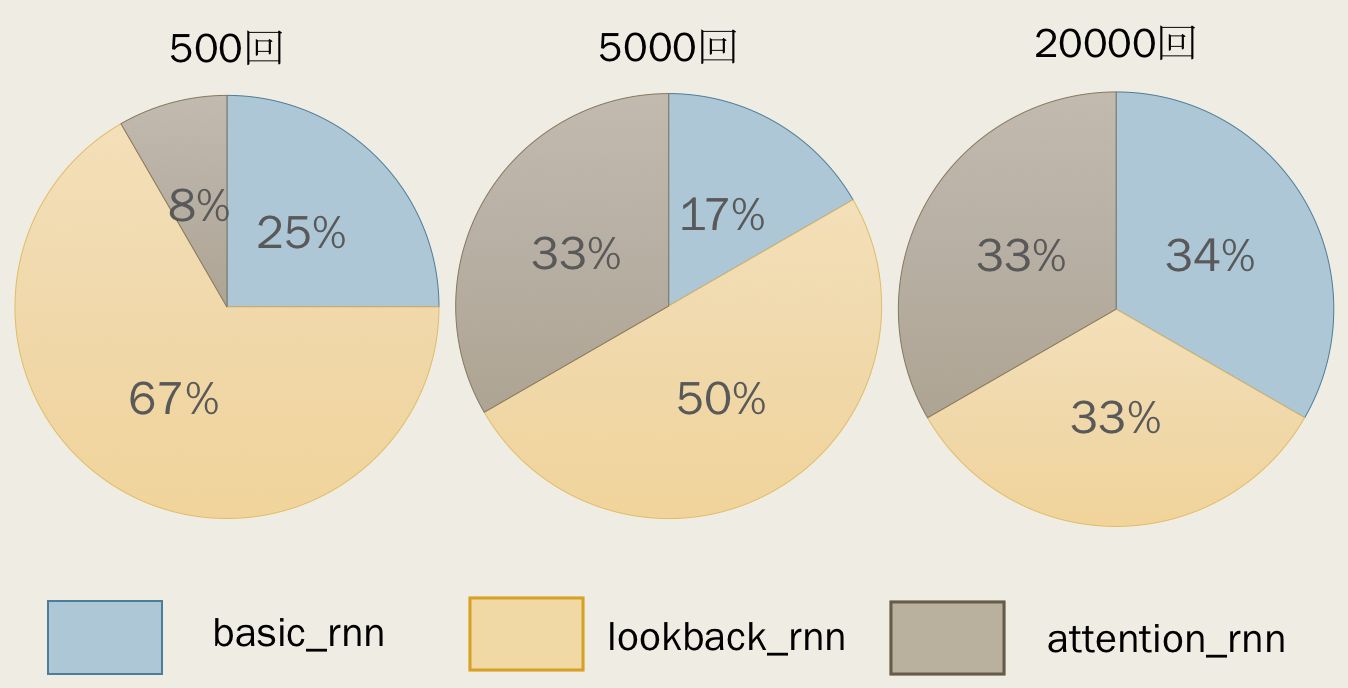
\includegraphics[scale=0.6, clip]{./img/glaph1.png}
        \caption{学習回数ごとの各モデルの調査結果}
        \label{fig:学習回数ごと各モデルの調査結果}
    \end{center}
    \end{screen}
\end{figure}
\newpage
\subsection{各モデルごとの学習回数の調査結果}
basic\_rnnでは学習回数が多い方が良いと答える人の割合が増えた.一方でattention\_rnnでは学習回数が500回のものが一番良いと答えた人の割合が増えた.\\
 以下の図\ref{fig:各モデルごとの学習回数の調査結果}に各モデルごとの学習回数の調査結果を示す.
\begin{figure}[h]
    \begin{screen}
    \begin{center}
        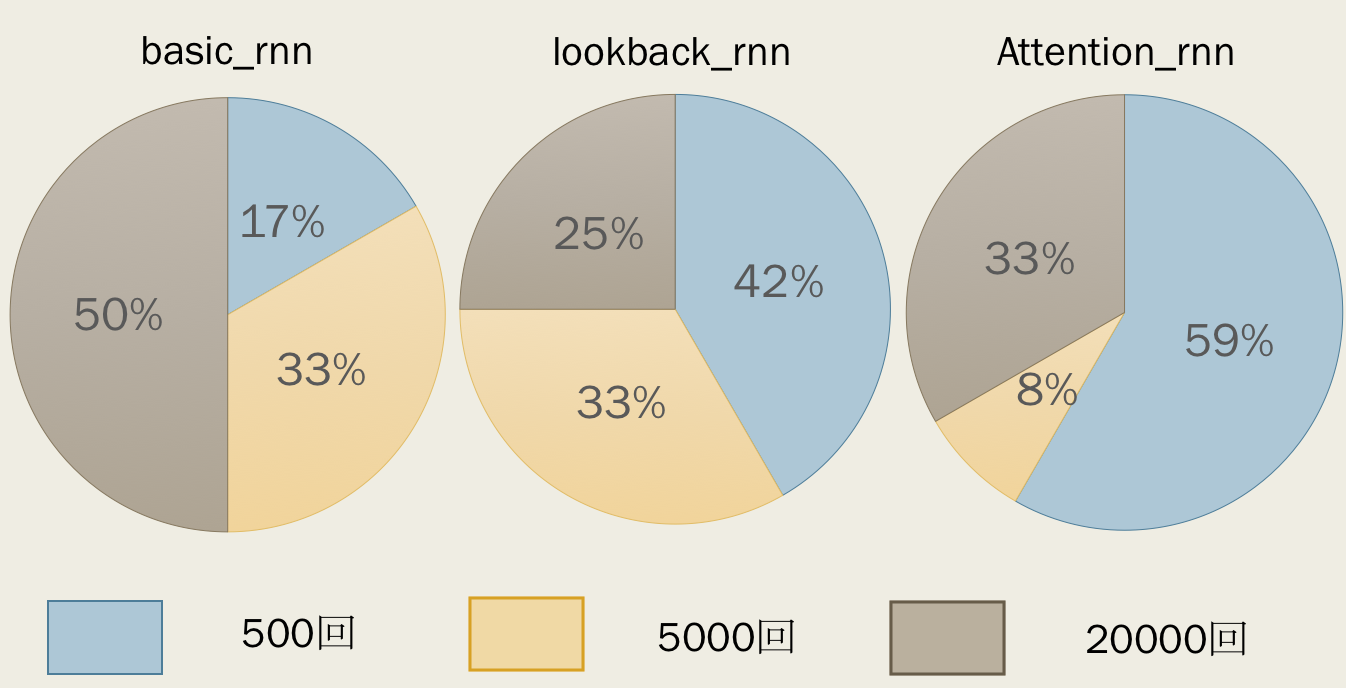
\includegraphics[scale=0.6, clip]{./img/glaph2.png}
        \caption{各モデルごとの学習回数の調査結果}
        \label{fig:各モデルごとの学習回数の調査結果}
    \end{center}
    \end{screen}
\end{figure}
\newpage
\subsection{ノード数ごとの調査結果}
ノード数ごとの調査結果ではノード数が128で生成したものが良いと答えた人の割合が一番多かった.これはノード数が多い方が長い音が増えたことや音階にまとまりが出たことで視聴者が聴きやすいと感じやすかったからだと考えられる.\\
 以下の図\ref{fig:ノード数の調査結果}にノード数の調査結果を示す.\\
\begin{figure}[h]
    \begin{screen}
    \begin{center}
        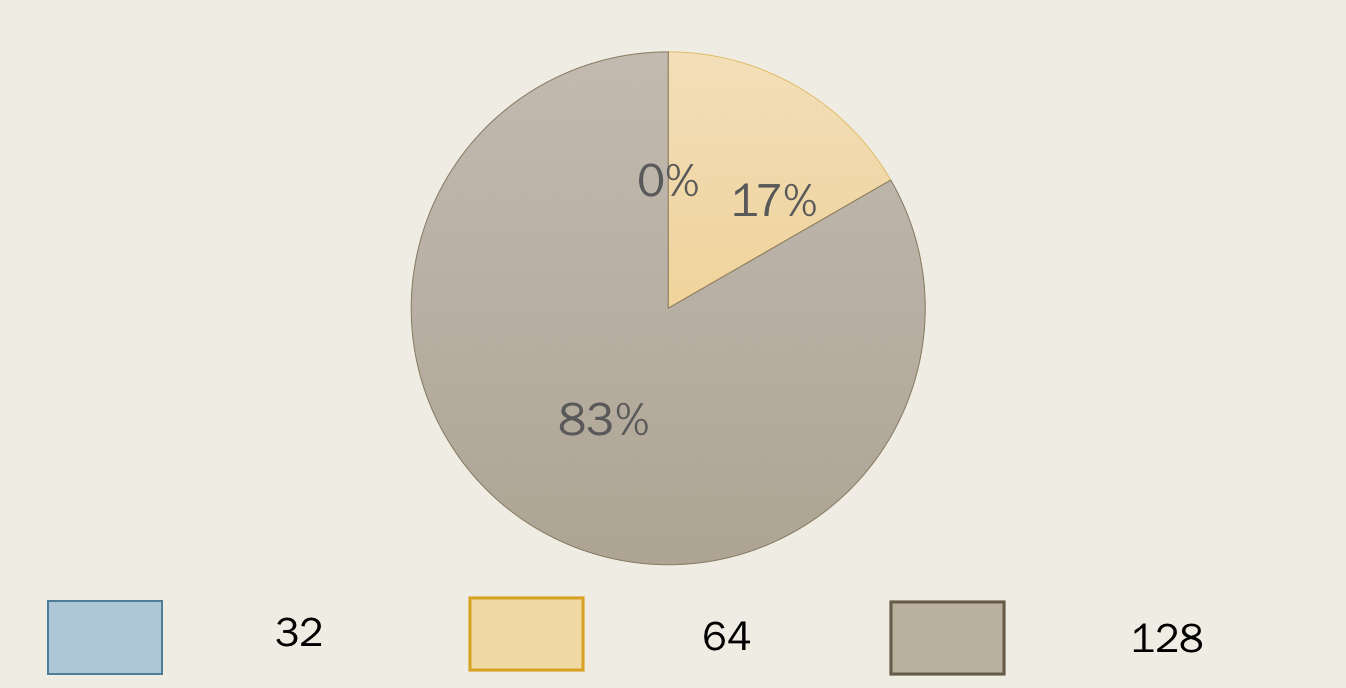
\includegraphics[scale=0.6, clip]{./img/glaph3.png}
        \caption{ノード数ごとの調査結果}
        \label{fig:ノード数の調査結果}
    \end{center}
    \end{screen}
\end{figure}
\newpage
\newpage
\section{今後の課題}
今回,様々な条件で楽曲を制作した.特に学習回数を大きくすると楽曲の精度は高まった.しかし音階やスケールは理解できているようだが,メロディに関してはあまり良いものとは言えなかった.要因としては学習に用いる楽曲が少なかったことや学習回数がまだ足りなかったことがあげられる.\\
 また,本実験の調査の結果からAIにおける楽曲制作において,必ずしもAIの学習回数を上げれば視聴者に有用な楽曲が生成されるわけではないことがわかった.これは人によって良いと感じる音やメロディ,リズムには差があり,AIによる正確性があれば良いと一概には言えないためだと思われる。
これは学習させる楽曲が一番影響を与えており,これを変えることで実験結果は変わると思われる.